\documentclass[10pt]{article}

\usepackage[letterpaper,margin=1in]{geometry}
\usepackage{amsmath,amssymb,amsthm}
\usepackage{newtxtext,newtxmath}
\usepackage{microtype}
\usepackage{graphicx}
\usepackage{booktabs}
\usepackage{array}
\usepackage{mathtools}
\usepackage{enumitem}
\usepackage{caption}
\usepackage{subcaption}
\usepackage{float}
\usepackage{lineno}
\usepackage{lastpage}
\usepackage{fancyhdr}
\usepackage{xcolor}
\usepackage{siunitx}
\usepackage{csquotes}
\usepackage[hidelinks]{hyperref}
\usepackage[
  backend=biber,
  style=authoryear,
  sorting=nyt,
  maxcitenames=2,
  maxbibnames=99,
  giveninits=false,
  uniquename=false,
  doi=true,
  url=false,
  isbn=false
]{biblatex}
\addbibresource{references.bib}

\setlength{\parindent}{0.22in}
\setlength{\parskip}{0pt}
\setlength{\bibitemsep}{3pt}
\setlist[itemize]{leftmargin=0.22in,itemsep=1pt,topsep=2pt}
\setlist[enumerate]{leftmargin=0.26in,itemsep=1pt,topsep=2pt}
\captionsetup{font=small,labelfont=bf}
\renewcommand{\arraystretch}{1.12}

\pagestyle{fancy}
\fancyhf{}
\fancyfoot[C]{\thepage}
\renewcommand{\headrulewidth}{0pt}

\modulolinenumbers[1]
\pagewiselinenumbers

\newtheorem{proposition}{Proposition}
\newtheorem{remark}{Remark}

\newcommand{\vect}[1]{\boldsymbol{#1}}
\newcommand{\R}{\mathbb{R}}
\newcommand{\T}{\mathsf{T}}
\newcommand{\Load}{\mathcal{L}}
\newcommand{\Beh}{\mathcal{B}_{\theta}}
\newcommand{\Acc}{\mathcal{A}}

\title{\textbf{A Typed Multi-Axis Mobility Tensor for Integrated Activity-Tour Choice and Congested Network Assignment}}
\author{}
\date{}

\begin{document}
\linenumbers

% ------------------------------------------------------------------
% TITLE PAGE
% ------------------------------------------------------------------
\begin{titlepage}
\thispagestyle{fancy}
\centering
\vspace*{0.35in}
{\Large\bfseries A Typed Multi-Axis Mobility Tensor for Integrated Activity-Tour Choice and Congested Network Assignment\par}
\vspace{0.45in}

{\large Xuesong Zhou, Ph.D.\par}
Professor, School of Sustainable Engineering and the Built Environment\\
Arizona State University, Tempe, Arizona 85287-3005\\
Email: \href{mailto:xzhou74@asu.edu}{xzhou74@asu.edu}\\
\vspace{0.25in}

{\large Ram M. Pendyala, Ph.D.\par}
Director and Professor, School of Sustainable Engineering and the Built Environment\\
Arizona State University, Tempe, Arizona 85287-3005\\
Email: \href{mailto:ram.pendyala@asu.edu}{ram.pendyala@asu.edu}\\
\vspace{0.25in}

\textit{Additional coauthors and affiliations may be inserted before submission.}

\vfill
\begin{tabular}{ll}
Corresponding author: & Xuesong Zhou\\
Submission type: & TRB Annual Meeting full paper draft\\
Total pages: & \pageref{LastPage}\\
\end{tabular}

\vspace{0.35in}
{\small Draft prepared for technical development and author review. Numerical findings use an explicitly identified synthetic prototype and certified open-source computational cases; they are not empirical validation results. Every number in this paper is regenerated by one script in the companion repository.}
\end{titlepage}
\setcounter{page}{2}

% ------------------------------------------------------------------
% STRUCTURED ABSTRACT
% ------------------------------------------------------------------
\newpage
\section*{Structured Abstract}

\textbf{Objectives.}
Sequential land-use, activity-based, and network assignment models exchange files and feedback loops, which obscures whether activity choices, origin-destination movements, and network flows are mathematically consistent at any iteration. This study develops a typed multi-axis mobility-tensor formulation in which one common vector of complete activity-tour-path columns generates mutually consistent tour, origin-destination, network-flow, and spatial-activity marginals, and in which integration is defined as shared column space and shared curvature rather than software coupling.

\textbf{Methods.}
A typed state and operator system assigns every axis, measure, and operator orientation an explicit contract. Complete columns jointly encode traveler class, activity-tour alternative, selected destinations, tour legs, and network paths. Sparse projections $\vect y=E\vect f$, $\vect q=R\vect f$, $\vect x=\Delta\vect f$, and $\mathcal X=\Gamma\vect f$ arise from one flow vector. Measured land-use opportunity supply $U_{ijm}$ restricts feasible destinations, enters tour attractiveness, and prices opportunity utilization. The behavior--network fixed point $\vect f^{\star}=\Beh[\,c(\Delta\vect f^{\star});U\,]$ closes the chain. The joint gradient and Hessian decompose into congestion, tour-choice, and opportunity curvature, yielding a second-order price for finite replacements of complete columns that is verified against exact objective changes. All computations run in an open-source certified package.

\textbf{Findings.}
On a 5-by-5 prototype with 1,000 travelers and 68 complete columns, 52.1\% selected work location W1 and 43.4\% selected a shopping tour in the base case. Shifting measured employment toward W2 raised its share from 47.9\% to 61.2\%. A 40\% central-capacity reduction raised the maximum volume-to-capacity ratio from 0.75 to 1.03 and reduced shopping-tour participation from 43.4\% to 41.4\%. For 500 feasible column replacements, mean absolute prediction error fell from 1.145 (first order) to 0.004 (second order), and the second-order remainder decayed cubically (median ratio 8.1 on step doubling; theory predicts 8). The same certified column-generation solver scales from the prototype grid to a 93,135-OD network with full-network-priced relative gaps below $10^{-4}$.

\textbf{Novelty.}
The framework contributes (i) a typed tensor and operator system with explicit measure and orientation contracts, (ii) integration defined as shared column-space consistency and shared curvature, and (iii) joint second-order pricing of complete activity--destination--path changes with a certified finite-move error analysis.

\textbf{Practical Applications.}
The formulation provides an inspectable prototype for testing how measured employment, retail, or service opportunities interact with destination selection, tour formation, congestion, and network investments, with a certified computational path from a hand-checkable grid to regional networks.

\newpage

% ------------------------------------------------------------------
\section{Introduction}
Activity-based travel demand models represent travel as a consequence of participation in activities organized into tours and daily schedules \parencite{pendyala1998,bowman2001}. Congested and dynamic network models represent the spatial realization of these choices through path flows, queues, and time-dependent link conditions \parencite{peeta2001,zhou2014}. Integrated land-use--transport systems add a third domain: the spatial distribution and capacity of the opportunities that make activity destinations feasible and attractive \parencite{pendyala2012}. Each domain is mature, yet practical integration commonly remains a sequence of files and feedback loops. Such coupling can obscure whether activity choices, origin-destination movements, and network flows are mathematically consistent at a given iteration, and it provides no joint sensitivity: no single object states how a change in one traveler's complete day propagates through shared congestion, shared tour alternatives, and shared opportunities.

This paper defines integration differently: as \emph{shared column-space consistency} and \emph{shared curvature}. One common vector of complete activity-tour-path columns generates every marginal the planner inspects, and one joint Hessian states every interaction among complete travel decisions. The formulation is developed inside a typed state and operator system in which each axis, each measure, and each operator orientation carries an explicit contract, so that behaviorally different quantities can never be silently aggregated.

The paper follows the six-stage architecture of Figure~\ref{fig:framework}:
\begin{equation}
\text{Represent}\rightarrow\text{Conserve}\rightarrow\text{Connect}\rightarrow\text{Stabilize}\rightarrow\text{Scale}\rightarrow\text{Transfer}.
\label{eq:sixstage}
\end{equation}
Represent: a typed mobility tensor with named axes (Section 2). Conserve: person, tour, leg, arc, and activity totals as exact projections of one flow (Section 2). Connect: land use $\rightarrow$ activity choice $\rightarrow$ tour $\rightarrow$ path $\rightarrow$ network as an operator chain (Section 3). Stabilize: the behavior--network fixed point and its joint Newton correction (Sections 3--4). Scale: sparse operators and certified column generation (Section 6). Transfer: GMNS-based regional implementation, treated as the practical extension (Section 7). The first four stages are developed carefully; one scaling experiment is reported; transfer is deliberately left as an extension.

\begin{figure}[H]
\centering
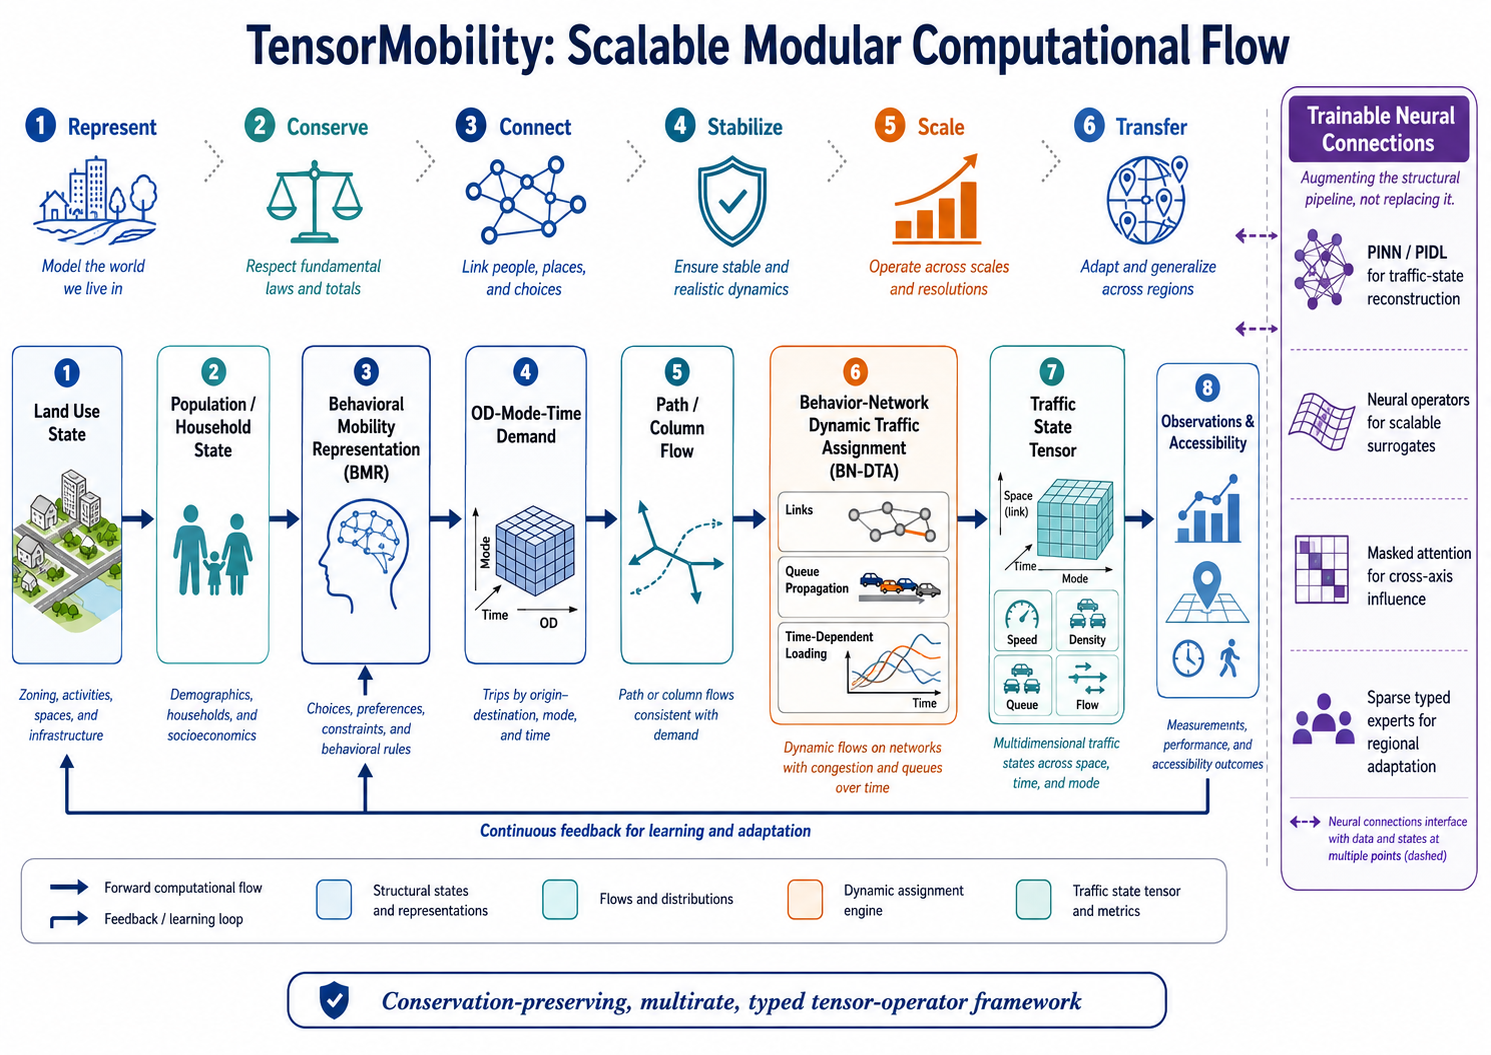
\includegraphics[width=0.97\textwidth]{figures/fig1_framework.png}
\caption{The integrated architecture: represent, conserve, connect, stabilize, scale, transfer. The present paper develops the first four stages for the activity-tour mobility tensor and reports one certified scaling experiment.}
\label{fig:framework}
\end{figure}

The contribution is not the use of a tensor and not the use of a grid. It is:
\begin{enumerate}
\item one typed state and operator system with explicit measure and orientation contracts;
\item one common column-flow representation from which all marginals are projections;
\item explicit synchronization between behavior and network loading, stated as a fixed point whose residual is never conflated with an equilibrium gap;
\item second-order pricing of complete activity--destination--path changes, with an exact finite-move verification and a cubic remainder law;
\item certified computation from a hand-checkable grid to networks with $10^{5}$ origin-destination pairs.
\end{enumerate}
Every numerical claim in this paper is regenerated by one script in the open-source companion repository (Section 6.4).

The word \emph{tensor} is used in its standard sense of a multidimensional array \parencite{kolda2009}; no tensor decomposition is required. The benefit is organizational: named axes preserve row, column, activity, and later time, without flattening their meanings prematurely.

% ------------------------------------------------------------------
\section{Typed Mobility Tensor and Complete Columns}

\subsection{The Typed State and the Paper Slice}
An integrated urban system carries a very large joint state; in the companion framework it is written once as
\begin{equation}
\mathcal X[h,n,c,r,u,o,d,m,\tau,p,a,t,\rho],
\label{eq:grandstate}
\end{equation}
over household, person, activity pattern, tour, trip leg, origin-destination pair, mode, departure interval, path, arc, time, and regime axes. This expression is stated only to fix the general object; the paper never operates on it directly, because its axes play different mathematical roles---some are states, some are choices, some are constraints, some are generated by algorithms---and an anonymous array erases those roles. What is required is a \emph{typed} tensor: every axis is named and registered, every mass-carrying vector declares its measure (probability, person flow, vehicle flow, state), and every operator declares source axis, target axis, and orientation
\begin{equation}
\vect y_{\text{target}} = M[\text{target}\leftarrow\text{source}]\;\vect x_{\text{source}}.
\label{eq:orientation}
\end{equation}
The type system is the mathematics: a contraction that violates a measure or orientation contract is rejected, not silently computed.

The paper then specializes \eqref{eq:grandstate} to one slice sufficient for integrated activity-tour choice and congested assignment:
\begin{equation}
\mathcal F_{g,\tau,\pi},
\label{eq:slice}
\end{equation}
where $g$ indexes traveler or household groups, $\tau$ indexes departure period or tour timing, and $\pi$ indexes \emph{complete activity--destination--path columns}. Each column is a complete realization
\begin{equation}
\pi=\big(\text{activity pattern},\ \text{destinations},\ \text{tour legs},\ \text{mode},\ \text{departure choice},\ \text{network paths}\big),
\label{eq:column}
\end{equation}
with flow $f_{\pi}\geq 0$. In the peak-period prototype the timing axis has one interval and the mode is fixed, so the flow vector $\vect f$ stacks $(g,\pi)$; the axes remain declared so that the temporal and modal extensions change the registry, not the formulation.

Demand conservation is imposed per group:
\begin{equation}
B\vect f=\vect q,\qquad
B[\text{group}\leftarrow\text{column}],
\label{eq:demand_conservation}
\end{equation}
where row $g$ of $B$ indicates the columns available to group $g$ and $q_g$ is its demand.

\subsection{Sparse Projections of One Common Flow}
Four typed projections generate every marginal from the common flow:
\begin{equation}
\vect y=E\vect f,\qquad
\vect q^{\mathrm{leg}}=R\vect f,\qquad
\vect x=\Delta\vect f,\qquad
\mathcal X=\Gamma\vect f.
\label{eq:projections}
\end{equation}
Here $E[\text{tour}\leftarrow\text{column}]$ maps each column to its activity-tour alternative (mass preserving); $R[\text{leg-OD}\leftarrow\text{column}]$ counts one unit per tour leg, producing the origin-destination demand that a trip-based model would treat as input; $\Delta[\text{arc}\leftarrow\text{column}]$ accumulates arc usage over all legs; and $\Gamma[\text{state}\leftarrow\text{column}]$ lifts the flow to the mobility tensor over grid-activity states $s=(i,j,m)$:
\begin{equation}
\mathcal X=[X_{ijm}]\in\R_+^{I\times J\times |\mathcal M|},
\qquad \mathcal M=\{H,W,S\}
\label{eq:basic_tensor}
\end{equation}
in the prototype (home, work, shopping). When temporal resolution is required, a stage or time axis extends the registry:
\begin{equation}
\mathcal X^{T}=[X_{ijmt}]\in\R_+^{I\times J\times |\mathcal M|\times |\mathcal T|},
\label{eq:temporal_tensor}
\end{equation}
with marginals $X^{S}_{ij}=\sum_m X_{ijm}$, $X^{M}_{m}=\sum_{i,j}X_{ijm}$, and $X^{T}_{t}=\sum_{i,j,m}X_{ijmt}$. Figure~\ref{fig:typed_tensor} shows the computed base-case tensor and its illustrative tour-stage extension.

\begin{figure}[H]
\centering
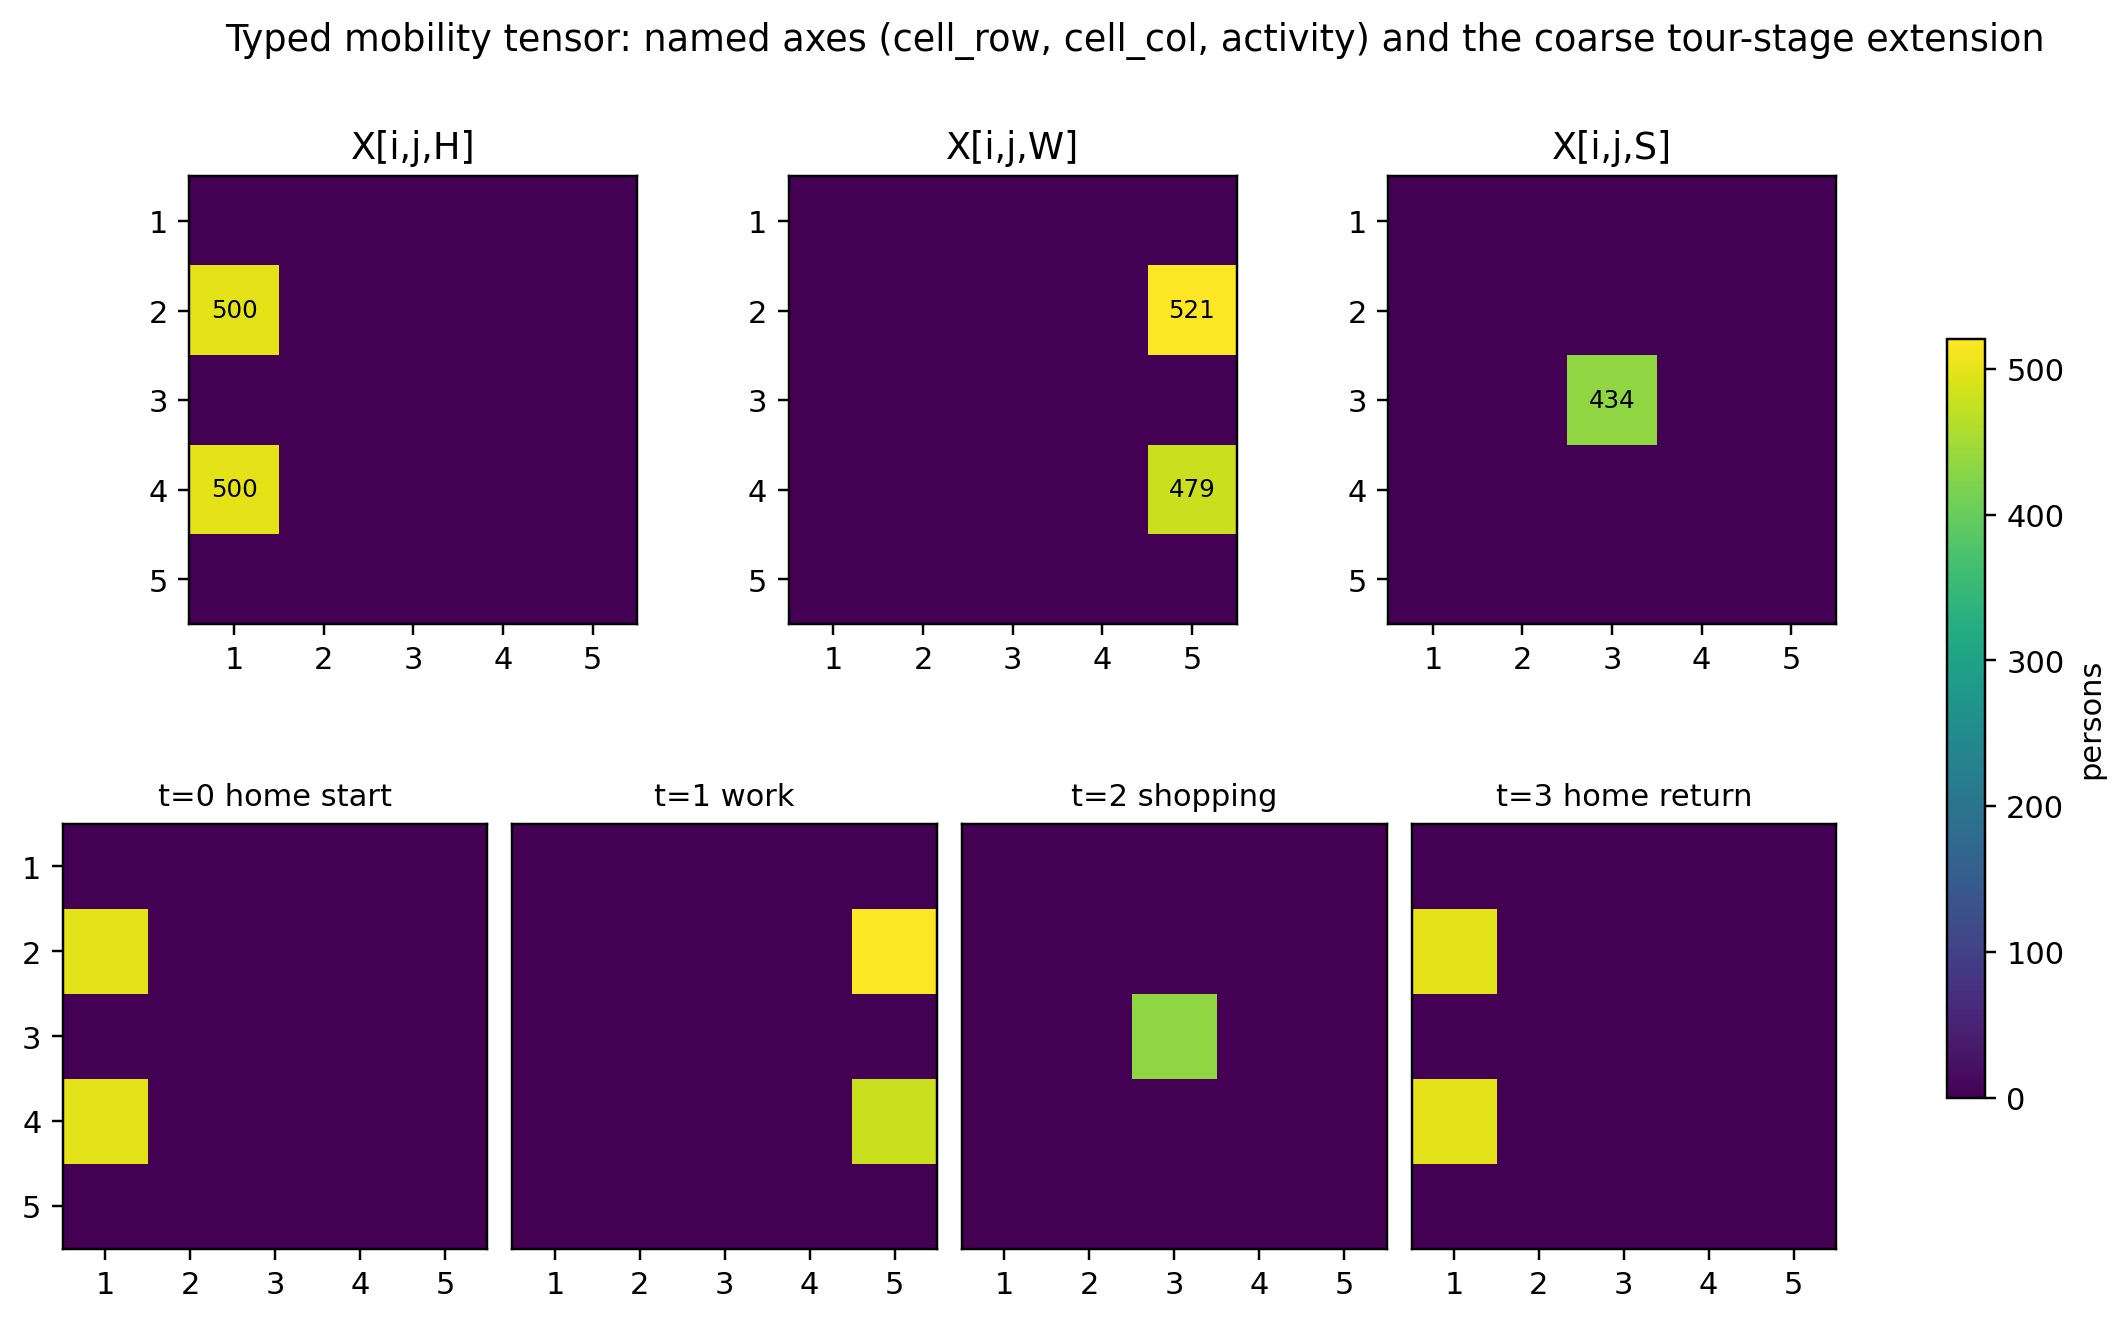
\includegraphics[width=0.99\textwidth]{figures/fig2_typed_tensor.png}
\caption{The typed mobility tensor of the solved base case: activity layers $X_{ijH}$, $X_{ijW}$, $X_{ijS}$ (top) and the coarse tour-stage extension $X_{ijmt}$ (bottom; an illustrative visualization, not a dynamic loading result). Axes are named and registered; the tensor is a projection $\mathcal X=\Gamma\vect f$, never an independent table.}
\label{fig:typed_tensor}
\end{figure}

\begin{proposition}[Integrated consistency]
If $\vect f$ satisfies \eqref{eq:demand_conservation}, then $\vect y$, $\vect q^{\mathrm{leg}}$, $\vect x$, and $\mathcal X$ generated by \eqref{eq:projections} are mutually consistent projections of the same activity-tour-path solution.
\end{proposition}

\begin{proof}
All four objects are linear images of the same feasible vector $\vect f$. Any unit of flow contributing to a tour, a leg, an arc, or an activity state originates from the same complete column and cannot be independently created in another model block.
\end{proof}

The grid is a transparent indexing device, not a claim of Manhattan geometry: real links may later be mapped to cells or replaced by an arbitrary network while the activity and tensor mappings are retained.

% ------------------------------------------------------------------
\section{Integrated Behavior--Network System}

\subsection{Measured Opportunity Supply $U$}
Let
\begin{equation}
U_{ijm}\geq 0
\label{eq:opportunity}
\end{equation}
be the measured land-use / activity-opportunity supply for activity $m$ at cell $(i,j)$: households for home, jobs for work, retail or service intensity for shopping. The symbol $U$ is reserved for this measured field; $\Load$ is reserved for the network loading operator, so the two never collide. The feasible support of activity $m$ is $\mathcal D_m=\{(i,j):U_{ijm}>0\}$, and a tour is feasible only if every activity destination belongs to its support.

Supply enters the model twice. First, it enters the linear attractiveness of a complete column,
\begin{equation}
a_{\pi}(U)=a^{0}_{\pi}
-\sum_{k=1}^{K}\alpha_{m_k}
\log\!\left(U_{i_kj_km_k}+\epsilon\right),
\label{eq:attractiveness}
\end{equation}
summed over the column's non-home activities. Second, it limits or prices aggregate use. With activity capacity $K_{ijm}=\kappa_m U_{ijm}$, a smooth opportunity-utilization potential is
\begin{equation}
\Phi_U(\mathcal X;U)=
\frac{\lambda_U}{2}\sum_{i,j,m}
\frac{X_{ijm}^2}{K_{ijm}+\epsilon},
\label{eq:opportunity_potential}
\end{equation}
representing competition for common work, shopping, or service opportunities. The field $U$ is measured and exogenous throughout this paper; annual land-use evolution belongs to a second, slower clock and is treated as an extension (Section 7).

\subsection{The Central Operator Chain}
The paper contains one main mathematical chain:
\begin{equation}
U
\;\xrightarrow{\;\Acc\;}\;
\text{accessibility, destination utilities}
\;\xrightarrow{\;\Beh\;}\;
\vect f
\;\xrightarrow{\;E,R,\Delta,\Gamma\;}\;
(\vect y,\vect q^{\mathrm{leg}},\vect x,\mathcal X)
\;\xrightarrow{\;\Load\;}\;
c(\vect x)
\;\xrightarrow{\;\Beh\;}\;
\vect f^{+}.
\label{eq:chain}
\end{equation}
$\Acc$ maps measured supply and travel costs to logsum accessibility and destination utilities; $\Beh$ is the behavior operator (activity pattern, tour, destination, and path choice at dispersion $\theta$); the four projections are the sparse operators of Section 2; and $\Load$ is congestion or dynamic loading, which in the static prototype reduces to arc cost $c(\vect x)$ with $\vect x=\Delta \vect f$. In compact form, the behavior--network state is the fixed point
\begin{equation}
\vect f^{\star}
=\Beh\!\left[\,c\!\left(\Delta\vect f^{\star}\right);\,U\,\right].
\label{eq:fixedpoint}
\end{equation}
This is the kernel of integrated activity-based demand and network assignment. The mobility tensor is not another model to be reconciled with it; it is the typed projection $\mathcal X=\Gamma\vect f^{\star}$.

Figure~\ref{fig:grid_tours} shows the prototype instantiation: the grid, the measured $U$ field, and the highest-flow complete home--work--home and home--work--shop--home columns of the solved base case.

\begin{figure}[H]
\centering
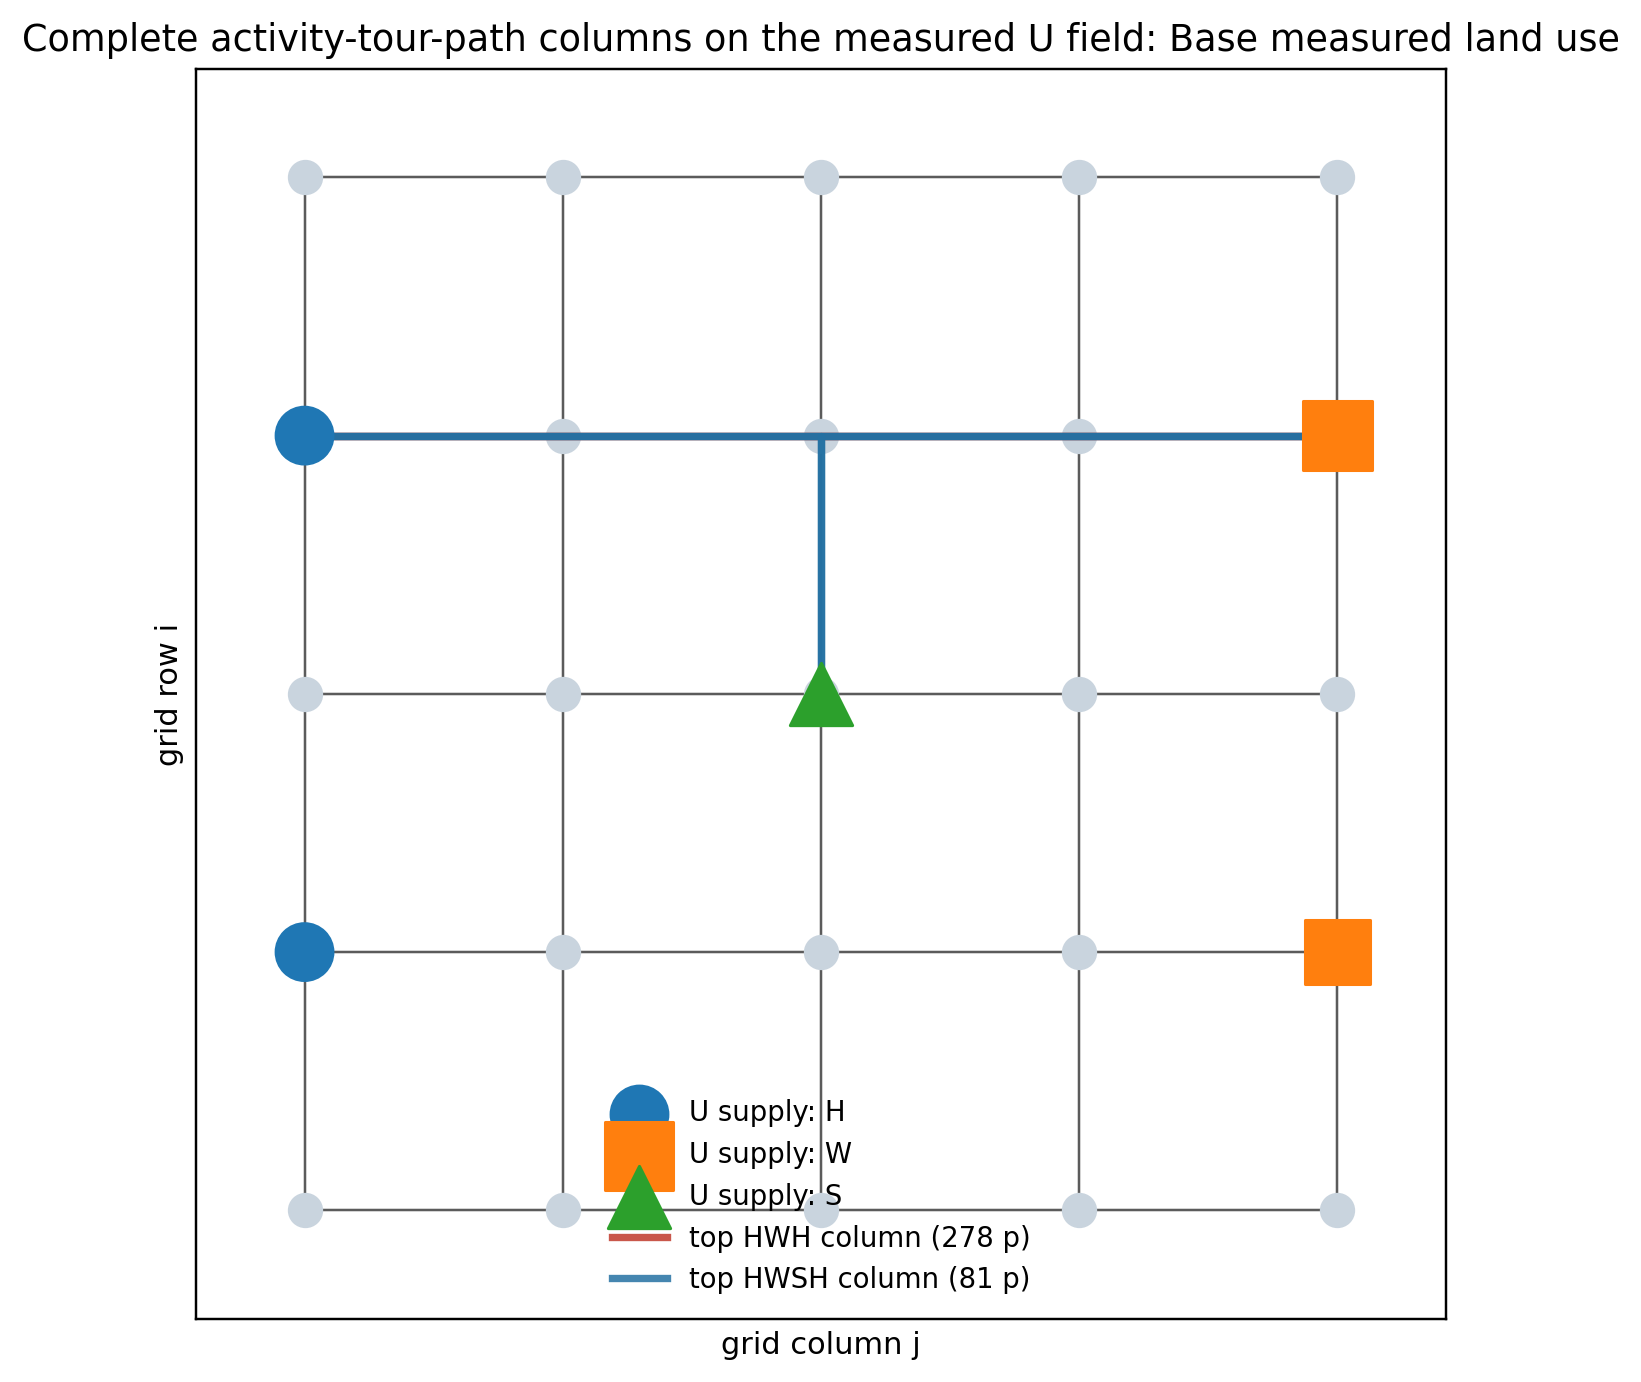
\includegraphics[width=0.82\textwidth]{figures/fig3_grid_tours.png}
\caption{Complete activity-tour-path columns on the measured opportunity field $U$. A column is not an origin-destination path; it is a complete tour realization with all legs. The two highlighted columns are the highest-flow HWH and HWSH alternatives at the solved base case.}
\label{fig:grid_tours}
\end{figure}

\subsection{Residual Discipline}
Integration claims require named residuals, and this paper keeps four distinct:
\begin{itemize}
\item the \emph{full-space relative gap} certifies static assignment: total cost minus all-origin shortest-path cost, priced over the full network, never over the enumerated pool;
\item the \emph{fixed-point residual} measures behavior--loading consistency in \eqref{eq:fixedpoint} when $\Load$ is a dynamic queue model; it is not a Wardrop gap and is never reported as one;
\item the \emph{conservation residual} certifies the projection stack \eqref{eq:projections} and demand constraint \eqref{eq:demand_conservation};
\item the \emph{exact finite-move error} evaluates pricing quality (Section 4), always against the true objective change, never against another approximation.
\end{itemize}
In the convex prototype, stationarity is certified as a KKT equal-gradient spread over positive columns within each group.

% ------------------------------------------------------------------
\section{Joint Second-Order Pricing}

\subsection{Integrated Objective, Gradient, and Hessian}
Collecting the linear costs $\vect a(U)$ from \eqref{eq:attractiveness}, a nondecreasing arc cost $c_a(x_a)$ with potential $\Phi_N(\vect x)=\sum_a\int_0^{x_a}c_a(u)\,du$, and a convex tour-choice dispersion $\Phi_M(\vect y)=\theta\sum y(\log y-1)$, the integrated model is
\begin{align}
\min_{\vect f\geq 0}\quad
F(\vect f;U)
={}&
\vect a(U)^\T\vect f
+\Phi_N(\Delta\vect f)
+\Phi_M(E\vect f)
+\Phi_U(\Gamma\vect f;U)
\label{eq:objective}\\
\text{s.t.}\quad &B\vect f=\vect q.
\label{eq:master_constraint}
\end{align}
Its gradient assigns every complete column one marginal value combining attractiveness, congested path cost, tour-choice pressure, and opportunity utilization:
\begin{equation}
\vect g
=\vect a(U)+\Delta^\T\vect c(\vect x)
+E^\T\nabla\Phi_M(\vect y)
+\Gamma^\T\nabla\Phi_U(\mathcal X;U).
\label{eq:gradient}
\end{equation}
With diagonal curvatures $D_N=\operatorname{diag}(c_a'(x_a))$, $D_M=\nabla^2\Phi_M(\vect y)$, and $D_U=\nabla^2_{\mathcal X}\Phi_U(\mathcal X;U)$, the joint Hessian is
\begin{equation}
H
=\Delta^\T D_N\Delta
+E^\T D_M E
+\Gamma^\T D_U\Gamma.
\label{eq:hessian}
\end{equation}
Column interaction therefore has exactly three sources: shared congested arcs, shared activity-tour alternatives, and shared land-use opportunities. Figure~\ref{fig:operator_hessian} shows the sparse projection stack and the assembled Hessian of the prototype.

\begin{figure}[H]
\centering
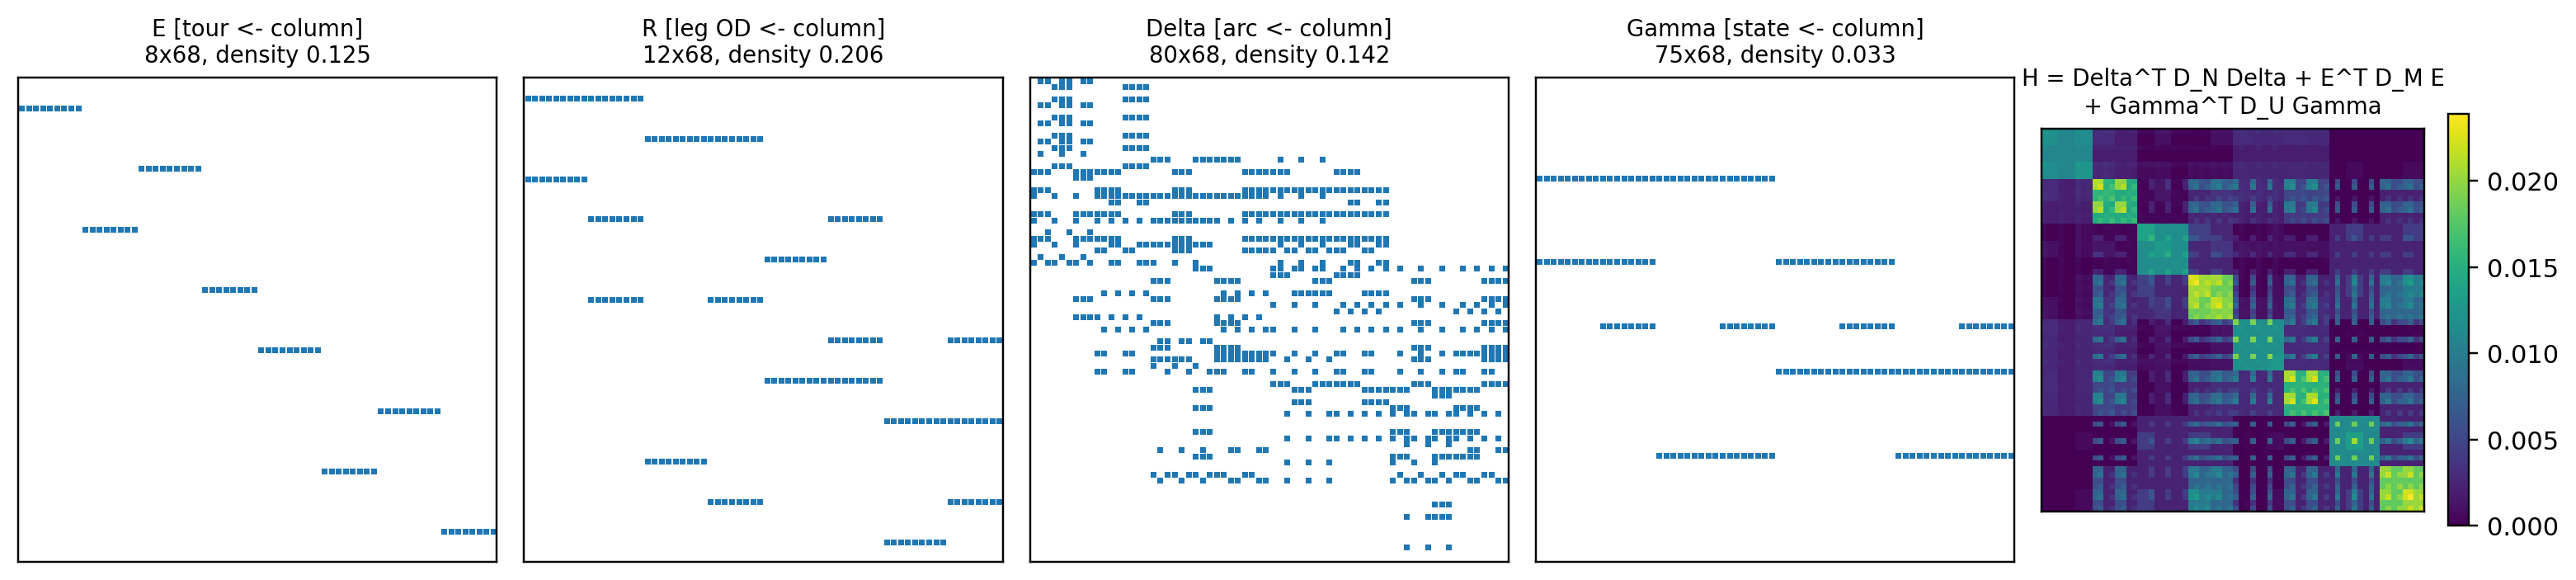
\includegraphics[width=0.99\textwidth]{figures/fig4_operator_hessian.png}
\caption{The typed projection stack $E$, $R$, $\Delta$, $\Gamma$ (sparsity patterns, orientation target $\leftarrow$ column) and the assembled joint Hessian $H=\Delta^\T D_N\Delta+E^\T D_M E+\Gamma^\T D_U\Gamma$ at the reference iterate.}
\label{fig:operator_hessian}
\end{figure}

\begin{proposition}[Convexity]
If every arc cost is nondecreasing and $\Phi_M$, $\Phi_U$ are convex on the feasible domain, then $H\succeq 0$ and \eqref{eq:objective}--\eqref{eq:master_constraint} is a convex continuous column-flow problem.
\end{proposition}

\begin{proof}
For any $\vect d$,
$\vect d^\T H\vect d
=(\Delta\vect d)^\T D_N(\Delta\vect d)
+(E\vect d)^\T D_M(E\vect d)
+(\Gamma\vect d)^\T D_U(\Gamma\vect d)\geq 0$
since each diagonal curvature is nonnegative; the constraints are linear.
\end{proof}

\subsection{Replacement Directions and the Second-Order Price}
At an iterate $\vect f^k$, the constrained Newton direction minimizes $Q_k(\vect d)=\vect g_k^\T\vect d+\tfrac12\vect d^\T H_k\vect d$ subject to $B\vect d=\vect 0$ and $\vect f^k+\vect d\geq 0$: a \emph{joint} change of complete columns, never a staged update of destination, tour, and path.

The elementary joint move replaces one complete column by another. For donor $\rho$ and candidate $\pi$ in the same group,
\begin{equation}
\vect d_{\pi\leftarrow\rho}
=\vect e_\pi-\vect e_\rho,
\label{eq:replacement}
\end{equation}
which preserves group mass exactly ($B\vect d_{\pi\leftarrow\rho}=\vect 0$). The second-order price of moving $\alpha$ travelers is
\begin{equation}
Q_{\pi\leftarrow\rho}(\alpha)
=\alpha\,\vect g^\T\vect d_{\pi\leftarrow\rho}
+\frac{\alpha^{2}}{2}\,
\vect d_{\pi\leftarrow\rho}^\T H
\vect d_{\pi\leftarrow\rho}.
\label{eq:second_order_price}
\end{equation}
The first term is the classical first-order (reduced-cost) price of column generation; the quadratic term prices what the first order cannot see: a candidate may be attractive because it avoids a shared bottleneck, shifts travelers toward an underused tour alternative, or uses an underutilized opportunity location. Because only the matrix-vector product $H\vect d$ is required, pricing one move never materializes column-pair interactions beyond the two moved columns.

\subsection{Exact Finite-Move Evaluation}
The second-order model is tested against the actual finite change, never only against another approximation:
\begin{equation}
\Delta F^{\mathrm{exact}}(\alpha)
=F(\vect f+\alpha\vect d)-F(\vect f),
\qquad
\Delta F^{(1)}=\alpha\,\vect g^\T\vect d,
\qquad
\Delta F^{(2)}=Q_{\pi\leftarrow\rho}(\alpha).
\label{eq:exact}
\end{equation}

\begin{proposition}[Cubic remainder]
If $F$ is three times continuously differentiable with $\|\nabla^3F\|\leq M_3$ along the segment $[\vect f,\vect f+\alpha\vect d]$, then
\begin{equation}
\left|\Delta F^{\mathrm{exact}}(\alpha)-\Delta F^{(2)}(\alpha)\right|
\leq \frac{M_3}{6}\,\alpha^{3}\,\|\vect d\|^{3}.
\label{eq:third_order}
\end{equation}
\end{proposition}

\begin{proof}
Taylor's theorem with Lagrange remainder applied to $\phi(\alpha)=F(\vect f+\alpha\vect d)$, whose third derivative is the third directional derivative of $F$ along $\vect d$.
\end{proof}

The bound creates a directly testable law: doubling the step must scale the remainder by a factor of eight. Section 6 verifies this on 500 sampled moves.

% ------------------------------------------------------------------
\section{Grid-Based Prototype}

\subsection{Network, Opportunities, and Columns}
The analytical example is intentionally small and fully enumerable. A bidirectional 5-by-5 grid has 25 nodes and 80 directed arcs; central row-3 / column-3 arcs have capacity 350, others 700, all with free-flow time 1. Two traveler groups, each of demand 500, originate at cells $(2,1)$ and $(4,1)$. Work opportunities are measured at W1$=(2,5)$ and W2$=(4,5)$; shopping at S$=(3,3)$. Each group chooses among four tour alternatives
\[
\text{H--W1--H},\quad \text{H--W2--H},\quad
\text{H--W1--S--H},\quad \text{H--W2--S--H},
\]
and for each tour leg two or three shortest simple paths are enumerated, producing 68 complete activity-tour-path columns, 12 tour-leg ODs, and 75 tensor states. Arc cost is the Bureau of Public Roads function $c_a(x_a)=t_a^0[1+0.15(x_a/C_a)^4]$. Opportunity capacities are 650 at W1, 550 at W2, 550 at S; the tour dispersion weight is $\theta=1.2$ and the opportunity weight $\lambda_U=1.2$. The prototype is a conceptual experiment, not a calibrated regional forecast.

\subsection{Scenarios and Protocol}
Three measured scenarios are solved with analytic gradients under group conservation:
\begin{enumerate}
\item \textbf{Base measured land use}: work supplies $(U_{W1},U_{W2})=(1000,800)$;
\item \textbf{Employment shifted toward W2}: supplies $(600,1400)$, capacities $(400,800)$;
\item \textbf{Central capacity $-40\%$}: base land use, central-corridor capacity multiplied by 0.60.
\end{enumerate}
For the pricing test, 500 feasible transfers of $\alpha=10$ travelers are sampled between column pairs of the same group at the uniform-flow reference iterate, and both predictions are compared with the exact change \eqref{eq:exact}; the same seeded moves are re-priced at $\alpha=5$ for the remainder-decay law.

Each solved scenario carries four machine-checked certificates: group-demand conservation, flow nonnegativity, the KKT equal-gradient spread over positive columns, and positive semidefiniteness of $H$. All pass in the reported runs.

% ------------------------------------------------------------------
\section{Computational Evidence}

\subsection{Scenario Responses}
Table~\ref{tab:scenario_results} reports the scenario results (Figure~\ref{fig:evidence}a--b). Employment relocation produces the intended endogenous destination response: the W2 share rises by 13.3 percentage points. Because W2 becomes both more attractive and more capacious, the integrated objective falls even though average network time rises slightly---network travel time alone is not a complete measure of an activity-based land-use scenario. The central capacity reduction raises the maximum volume-to-capacity ratio above one and reduces shopping-tour participation by 1.9 percentage points; the response emerges because complete shopping tours use an additional leg that interacts with the bottleneck, not because a shopping reduction was prescribed.

\begin{table}[H]
\centering
\caption{Synthetic 5-by-5 prototype results (generated by the companion case script)}
\label{tab:scenario_results}
\small
\begin{tabular}{lrrrrrr}
\toprule
Scenario &
Obj./person &
Network time &
W1 share &
W2 share &
Shopping share &
Max.\ $v/c$\\
\midrule
Base measured land use
& 13.776 & 9.314 & 52.1\% & 47.9\% & 43.4\% & 0.75\\
Employment shifted to W2
& 13.687 & 9.412 & 38.8\% & 61.2\% & 44.5\% & 0.82\\
Central capacity $-40\%$
& 13.793 & 9.348 & 52.0\% & 48.0\% & 41.4\% & 1.03\\
\bottomrule
\end{tabular}
\end{table}

\subsection{Second-Order Pricing Accuracy}
Table~\ref{tab:pricing_results} and Figure~\ref{fig:evidence}c report the pricing experiment. The quadratic price reduces mean absolute error by 99.6\% relative to the first-order price, and the second-order prediction nearly overlays the exact finite change. The remainder law \eqref{eq:third_order} is confirmed directly: re-pricing the same 500 moves at half the step yields a median remainder ratio of 8.10 on step doubling, against the theoretical cubic factor of 8.

\begin{table}[H]
\centering
\caption{Prediction of exact objective change for 500 feasible column replacements ($\alpha=10$)}
\label{tab:pricing_results}
\small
\begin{tabular}{lrr}
\toprule
Metric & First-order pricing & Second-order pricing\\
\midrule
Mean absolute error & 1.1450 & 0.0041\\
Root mean squared error & 1.2703 & 0.0050\\
Spearman rank correlation & 0.999514 & 0.999995\\
\bottomrule
\end{tabular}
\end{table}

\subsection{Certified Scalability}
The prototype's assignment layer is not bespoke: the same certified column-generation solver runs from generated grids to standard networks, with every relative gap priced over the full network by all-origin shortest paths. Table~\ref{tab:scaling} reports a fresh single-thread run (Figure~\ref{fig:evidence}d). The Chicago Sketch row is quoted as optional practical evidence of transfer; regional TRMG2 and corridor datasets used elsewhere in the companion repository are locally held and deliberately excluded from this paper's evidentiary base.

\begin{table}[H]
\centering
\caption{Certified column-generation ladder (single thread; full-network-priced relative gap)}
\label{tab:scaling}
\small
\begin{tabular}{lrrrrrr}
\toprule
Network & Nodes & Links & OD pairs & Columns & Full-space gap & Wall (s)\\
\midrule
Grid $10\times10$ & 100 & 360 & 20 & 280 & $8.0\times10^{-5}$ & 0.2\\
Grid $20\times20$ & 400 & 1{,}520 & 60 & 2{,}750 & $9.8\times10^{-5}$ & 2.3\\
Grid $50\times50$ & 2{,}500 & 9{,}800 & 200 & 16{,}041 & $2.4\times10^{-4}$ & 24.6\\
Chicago Sketch & 933 & 2{,}950 & 93{,}135 & 198{,}683 & $9.8\times10^{-5}$ & 6.5\\
\bottomrule
\end{tabular}
\end{table}

\begin{figure}[H]
\centering

\includegraphics[width=0.99\textwidth]{figures/fig5_numerical_evidence.png}
\caption{Numerical evidence: (a) destination and tour response across measured scenarios; (b) peak congestion response; (c) first- versus second-order replacement pricing against exact objective changes; (d) the certified column-generation scalability ladder.}
\label{fig:evidence}
\end{figure}

\subsection{Reproducibility}
Every number in Tables~\ref{tab:scenario_results}--\ref{tab:scaling} and Figures~\ref{fig:typed_tensor}--\ref{fig:evidence} is generated by one script, \texttt{cases/run\_mobility\_tensor\_paper.py}, in the open-source TensorMobility repository (\url{https://github.com/asu-trans-ai-lab/TensorMobility}). The script exports the scenario tables, the pricing samples, the remainder-decay measurement, the scalability ladder, all figures, and a machine-readable \texttt{certificates.json}; the joint gradient, Hessian, and pricing calculus are unit-tested against finite differences and exact finite moves in the same repository.

% ------------------------------------------------------------------
\section{Limitations and Extensions}

\textbf{Two clocks.} The paper keeps the within-day clock (departure, loading) separate from the annual clock (land-use evolution). $U$ is measured and fixed here; annual stock-flow feedback, in which accessibility reshapes $U$, belongs to an outer loop and is an extension, not a hidden assumption.

\textbf{Dynamic loading.} In \eqref{eq:chain}, $\Load$ reduces to static arc costs. Replacing it with time-dependent queue loading changes the certificate from a convex-optimality gap to a fixed-point residual; the residual discipline of Section 3.3 is designed so that this replacement does not silently weaken the reported guarantees.

\textbf{Decomposition.} ADMM-style consensus \parencite{boyd2011} can coordinate the marginal blocks $\Phi_N$, $\Phi_M$, $\Phi_U$ at scale, but it is a solver choice, not the definition of integration, and dropping cross-block curvature changes the Newton direction \eqref{eq:second_order_price}. Decomposition therefore belongs to the computational layer and is used only when regional path sets or temporal layers make the joint quadratic subproblem large.

\textbf{Learned components.} Neural terms are admissible only as bounded residuals attached to the structural operators with a feasibility projection---structure first, learning as correction---and are deliberately excluded from this paper's kernel.

\textbf{Integer schedules.} The continuous model does not provide integer household schedules; branch-and-price extensions over the same column space require separate analysis.

\textbf{Transfer.} The sixth stage of \eqref{eq:sixstage} replaces grid cells with zones or parcels and grid arcs with GMNS multimodal networks; the typed operator contracts are unchanged. The certified ladder of Table~\ref{tab:scaling} indicates that the assignment layer scales; regional activity-tour column generation with measured $U$ fields is the natural next paper.

\textbf{Precautions.} A tensor by itself does not guarantee integration---the incidence mappings and conservation contracts do. Measured land-use intensity must be converted to attractiveness or capacity with transparent units. Synthetic results demonstrate mechanisms, not forecasting performance.

% ------------------------------------------------------------------
\section{Conclusion}
This paper presented a typed multi-axis mobility tensor embedded in a common activity-tour-path column space. One flow vector generates tour, leg-OD, arc, and spatial-activity marginals as typed projections; measured opportunity supply $U_{ijm}$ restricts destinations, enters attractiveness, and prices utilization; and the behavior--network state is the fixed point $\vect f^{\star}=\Beh[c(\Delta\vect f^{\star});U]$. Integration is thereby defined as shared column-space consistency and shared curvature:
\[
H=\Delta^\T D_N\Delta+E^\T D_M E+\Gamma^\T D_U\Gamma,
\]
in which columns interact only through shared arcs, shared tour alternatives, and shared opportunities. Joint second-order pricing of complete column replacements reduced finite-move prediction error by 99.6\% relative to first-order pricing and obeyed the cubic remainder law (median ratio 8.10 on step doubling), while the same certified solver carried the assignment layer from the hand-checkable grid to a 93,135-OD network at full-space gaps below $10^{-4}$.

The research proposition remains deliberately simple: the typed axes supply meaning, the complete column supplies consistency, the fixed point supplies synchronization, the Hessian supplies joint sensitivity, and the certificates make every claim executable.

% ------------------------------------------------------------------
\section*{Acknowledgments and Generative AI Disclosure}
The authors acknowledge the prior methodological foundations of activity-based modeling, integrated land-use--transport microsimulation, traffic assignment, and nonlinear optimization that motivate this framework.

Generative AI tools were used under author direction and review: OpenAI ChatGPT assisted with initial equation organization, LaTeX drafting, and conceptual illustration of an earlier draft; Anthropic Claude assisted with the present revision, with integrating the prototype into the open-source TensorMobility repository, and with drafting the reproducible case script and unit tests. The authors are responsible for independently reviewing and verifying all equations, references, numerical computations, interpretations, and final manuscript content. All reported numbers are regenerated by the cited open-source script.

\printbibliography[title={References}]

\end{document}
